\documentclass[pra, onecolumn, notitlepage, floats, 11pt]{revtex4-1}

\usepackage[T1]{fontenc}
\usepackage{graphicx}
\usepackage{color}
\usepackage{latexsym,amsmath}
\usepackage{comment}
\usepackage{tabularx}
\usepackage{siunitx}
\usepackage{multirow}
\usepackage{mathtools}
\usepackage{tikz, fp}
\usepackage{wrapfig}
\usepackage{amsfonts}
\usepackage[pdftex,colorlinks=true, pdfstartview=FitV, linkcolor=linkcolor, citecolor=linkcolor, urlcolor=linkcolor, hyperindex=true,hyperfigures=true]{hyperref} %hyperlink%
\usepackage{fancyhdr}
\usepackage{inconsolata}
\usepackage{listings}
\usepackage{physics}
\usepackage{datetime}
\usepackage[caption=false]{subfig}
\usepackage{titlesec}

\renewcommand{\figurename}{Figure}
\renewcommand{\tablename}{Table}
\renewcommand{\thetable}{\arabic{table}}

\definecolor{airforceblue}{rgb}{0.36, 0.54, 0.66}  %#5D8AA8
\definecolor{cobalt}{rgb}{0.0, 0.28, 0.67}         %#0047AB
\definecolor{coolblack}{rgb}{0.0, 0.18, 0.39}      %#002E63
\definecolor{dartmouthgreen}{rgb}{0.05, 0.5, 0.06} %#00693E
\definecolor{lava}{rgb}{0.81, 0.06, 0.13}          %#CF1020
% move section headings to left
% \sffamily
% \scshape
%\titleformat{\section}{\raggedright\sffamily\bfseries\fontsize{13pt}{13}\selectfont}{\arabic{section}}{1em}{\MakeUppercase}
\titleformat{\section}{\raggedright\bfseries\scshape\fontsize{13pt}{13}\selectfont}{\color{cobalt}\arabic{section}}{1em}{\color{cobalt}}
\titleformat{\subsection}{\raggedright\bfseries\scshape\fontsize{12pt}{12}\selectfont}{{\color{cobalt}\arabic{section}.\arabic{subsection}}}{1em}{\color{cobalt}}
\renewcommand{\thesection}{\arabic{section}}
\renewcommand{\thesubsection}{\arabic{subsection}}
\renewcommand{\thesubsubsection}{\arabic{subsubsection}}
\makeatletter
\renewcommand{\p@subsection}{\thesection.}
\renewcommand{\p@subsubsection}{\thesection.\thesubsection.}
\makeatother


\linespread{0.956}

\DeclarePairedDelimiter\ceil{\lceil}{\rceil}
\DeclarePairedDelimiter\floor{\lfloor}{\rfloor}

\definecolor{linkcolor}{rgb}{0,0,0.65}
\definecolor{shadecolor}{rgb}{0.95, 0.95, 0.95}
\definecolor{mygreen}{rgb}{0,0.6,0}
\definecolor{mygray}{rgb}{0.5,0.5,0.5}
\definecolor{mymauve}{rgb}{0.58,0,0.82}
\lstdefinestyle{fortran}
{
    backgroundcolor=\color{shadecolor},       % background color
    basicstyle=\ttfamily\footnotesize,        % the size of the fonts that are used for the code
    breakatwhitespace=false,                  % sets if automatic breaks should only happen at whitespace
    breaklines=false,                         % sets automatic line breaking
    captionpos=b,                             % sets the caption-position to bottom
    commentstyle=\color{mygreen},             % comment style
    extendedchars=true,                       % lets you use non-ASCII characters; for 8-bits encodings only, does not work with UTF-8
    keepspaces=true,                          % keeps spaces in text, useful for keeping indentation of code (possibly needs columns=flexible)
    keywordstyle=\bfseries\color{blue},       % keyword style
    language=[95]Fortran,                     % the language of the code
    numbers=left,                             % where to put the line-numbers; possible values are (none, left, right)
    numbersep=5pt,                            % how far the line-numbers are from the code
    numberstyle=\tiny\color{mygray},          % the style that is used for the line-numbers
    rulecolor=\color{black},                  % if not set, the frame-color may be changed on line-breaks within not-black text (e.g. comments (green here))
    showspaces=false,                         % show spaces everywhere adding particular underscores; it overrides 'showstringspaces'
    showstringspaces=false,                   % underline spaces within strings only
    showtabs=false,                           % show tabs within strings adding particular underscores
    stepnumber=1,                             % the step between two line-numbers. If it's 1, each line will be numbered
    stringstyle=\color{mymauve},              % string literal style
    tabsize=4,                                % sets default tabsize to 4 spaces
    title=\lstname                            % show the filename of files
}

\lstdefinestyle{python}
{
    backgroundcolor=\color{shadecolor},       % background color
    basicstyle=\ttfamily\footnotesize,        % the size of the fonts that are used for the code
    breakatwhitespace=false,                  % sets if automatic breaks should only happen at whitespace
    breaklines=false,                         % sets automatic line breaking
    captionpos=b,                             % sets the caption-position to bottom
    commentstyle=\color{mygreen},             % comment style
    extendedchars=true,                       % lets you use non-ASCII characters; for 8-bits encodings only, does not work with UTF-8
    keepspaces=true,                          % keeps spaces in text, useful for keeping indentation of code (possibly needs columns=flexible)
    keywordstyle=\bfseries\color{blue},       % keyword style
    language=Python,                          % the language of the code
    numbers=left,                             % where to put the line-numbers; possible values are (none, left, right)
    numbersep=5pt,                            % how far the line-numbers are from the code
    numberstyle=\tiny\color{mygray},          % the style that is used for the line-numbers
    rulecolor=\color{black},                  % if not set, the frame-color may be changed on line-breaks within not-black text (e.g. comments (green here))
    showspaces=false,                         % show spaces everywhere adding particular underscores; it overrides 'showstringspaces'
    showstringspaces=false,                   % underline spaces within strings only
    showtabs=false,                           % show tabs within strings adding particular underscores
    stepnumber=1,                             % the step between two line-numbers. If it's 1, each line will be numbered
    stringstyle=\color{mymauve},              % string literal style
    tabsize=4,                                % sets default tabsize to 4 spaces
    title=\lstname                            % show the filename of files
}


\pagestyle{fancy}
\fancyhf{}
\fancyhead[L]{Rocco Ardino (Mat. 1231629)}
\fancyhead[R]{\bf\thepage}
\fancyfoot[L]{\textsc{report}: Week 6}
\fancyfoot[R]{\today}
\renewcommand{\headrulewidth}{0.1pt}
\renewcommand{\footrulewidth}{0.1pt}

\newcommand{\codebold}[2][cobalt]{\texttt{\bfseries {\color{#1}#2}}}
\newcommand{\code}[2][black]{\color{#1}\texttt{#2}}
\newcommand{\codefunctionbold}[2]{\texttt{\bfseries {\color{cobalt}#1}({\color{lava}#2})}}
\newcommand{\codefunction}[2]{\texttt{#1(#2})}










\begin{document}

\title{Quantum Information and Computing 2020/21\\Week 6 report}

\author{Rocco Ardino}

\date{\today}





\begin{abstract}
    In this work we provide a numerical solution to the time independent Schr$\mathrm{\ddot{o}}$dinger equation for a monodimensional harmonic oscillator in a limited space interval. The method of finite differences is employed for the purpose and the results found for the first \( k \) eigenvalues are compared with the theory expectation. Lastly, the first eigenfunctions are plotted in order to check the correctness of the numerical simulation.
\end{abstract}

\maketitle




\section{Theory}
Schr$\mathrm{\ddot{o}}$dinger equation for a monodimensional quantum harmonic oscillator and for \( \hbar = 1 \) reads:
\begin{equation}
    H \psi_{n}
    =
    \qty(- \frac{1}{2m} \dv[2]{}{x} + \frac{1}{2} m \omega^2 x^2) \psi_{n}
    =
    E_{n} \psi_{n}
    \quad ,
    \label{eq:06_T_1}
\end{equation}
being \( E_{n} \) and \( \psi_{n} \) respectively the \( n^{\text{th}} \) eigenvalue and eigenfunction of the Hamiltonian \( H \). In particular, from theory we know that the eigenvalues read:
\begin{equation}
    E_{n}
    =
    \qty(n + \frac{1}{2}) \omega
    \quad ,
    \label{eq:06_T_2}
\end{equation}
with \( n \ge 0 \), and the eigenfunctions are linked to the Hermite functions \( H_{n}(x) \). In \( x \) representation:
\begin{equation}
    \psi_{n}(x)
    =
    \frac{1}{\sqrt{2^{n}n!}}
    \cdot
    \qty(\frac{m\omega}{\pi})^{\frac{1}{4}}
    \cdot
    e^{-\frac{m \omega x^2}{2}}
    \cdot
    H_{n}\qty(\sqrt{m \omega} x)
    \quad .
    \label{eq:06_T_3}
\end{equation}

Now, we focus on the technique to solve numerically this problem. For simplicity, let us limit on a finite and symmetric space interval \( [-a,a] \). Then, we discretize it into \( N \) smaller intervals of width \( \Delta x = \frac{2a}{N} \), which define the points \( x_{i} = -a + i\Delta x \), \( i = 0, \dots, N \). With such choice, the finite differences method applied to the second derivative of \( \psi \) evaluated in the point \( x_{i} \) returns:
\begin{equation}
    \dv[2]{\psi}{x} \qty(x_{i})
    =
    \frac{\psi\qty(x_{i+1}) - 2\psi\qty(x_{i}) + \psi\qty(x_{i-1})}{\qty(\Delta x)^2}
    \quad .
    \label{eq:06_T_4}
\end{equation}
These tricks translate our problem into a linear algebra one, namely finding the eigenvalues and eigenvectors of the following tridiagonal matrix, representing the discretized Hamiltonian:
\begin{equation}
    \displaystyle
    \begin{bmatrix}
        \displaystyle \frac{2}{2m\qty(\Delta x)^{2}} + \frac{1}{2}m\omega^{2} x_{0}^2  &
        \displaystyle - \frac{1}{2m\qty(\Delta x)^{2}}  &
        0   &
        \cdots  &
        0   \\
        \displaystyle - \frac{1}{2m\qty(\Delta x)^{2}}  &
        \displaystyle \frac{2}{2m\qty(\Delta x)^{2}} + \frac{1}{2}m\omega^{2} x_{1}^2  &
        \displaystyle - \frac{1}{2m\qty(\Delta x)^{2}}  &
        \cdots  &
        0   \\
        0   &   \displaystyle - \frac{1}{2m\qty(\Delta x)^{2}}  &
        %\displaystyle \frac{2}{2m\qty(\Delta x)^{2}} + \frac{1}{2}m\omega^{2} x_{2}^2  &
        \ddots  &
        \cdots  &
        0   \\
        \vdots  &
        \vdots  &
        \vdots  &
        \ddots  &
        \vdots  \\
        \cdots  &
        \cdots  &
        \cdots  &
        \cdots  &
        \displaystyle \frac{2}{2m\qty(\Delta x)^{2}} + \frac{1}{2}m\omega^{2} x_{N}^2
    \end{bmatrix}
    \quad .
    \label{eq:06_T_5}
\end{equation}





\section{Code Development}
For this work, the new module \codebold{sch\_eq\_utils} is implemented, containing several functions and subroutines for multiple purposes:
\begin{itemize}
    \item \codefunctionbold{init\_ham}{N,L,m,omega}, for instantiating the tridiagonal \( (N+1) \times (N+1) \) matrix expressed in Eq. \ref{eq:06_T_5}, considering a symmteric space interval of length \code{L} and with \code{m} and \code{omega} parameters;
    \item \codefunctionbold{diag\_ham}{ham,eigs}, for diagonalizing the tridiagonal matrix in Eq. \ref{eq:06_T_5} and returning the eigenvalues and eigenfunctions inside the appropriate input arguments, which are modified during the execution;
    \item \codefunctionbold{print\_eigfc}{xs,ys,filename,unit}, for printing on a certain file the discretized \( x_{i} \) and the corresponding \( \psi(x_{i}) \);
    \item \codefunctionbold{print\_eigvl}{xs,es,eigs,filename,unit}, for printing on a certain file the eigenvalues \( E_{i} \), computed from both numerical solution and theory, and the corresponding index \( i \).
\end{itemize}

In particular, we explain the core functionalities and the workflow in the following subsections.



\subsection{Discretized Hamiltonian initialization}
The code for the initialization of the discretized Hamiltonian matrix of Eq. \ref{eq:06_T_5} is showed in Listing \ref{lst:06_C_SS_1_1}. Note that the input parameters are the number of discrete intervals \( N \), the size \( L \) of the symmetric space interval \( [-a,a] \) and the parameters \( m \) and \( \omega \).

\medskip
\begin{lstlisting}[
    style=fortran,
    frame=single,
    label={lst:06_C_SS_1_1},
    caption={Implementation of the initialization of discretized Hamiltonian tridiagonal matrix.}
]
function init_ham(N, L, m, omega) result(ham)
    ! input arguments
    integer(4) :: N     ! hamiltonian dimesnions
    real(8)    :: L     ! width of the box
    real(8)    :: m     ! mass
    real(8)    :: omega ! omega

    real(8), dimension(N+1,N+1) :: ham
    real(8) :: DL
    integer(4) :: ii, jj

    DL = L / N
    do ii=1,N+1
        do jj=1,N+1
            if (ABS(ii-jj)==1) then
                ham(ii,jj) = - (1.0d0/(2.0d0*m)) * (1.0d0/(DL**2))
            else if (ii==jj) then
                ham(ii,jj) =   (1.0d0/(2.0d0*m)) * (2.0d0/(DL**2)) &
                             + (0.5d0*m*omega**2) * (-L/2 + DL*(ii-1))**2
            else
                ham(ii,jj) =    0.0d0
            end if
        end do
    end do
end function init_ham
\end{lstlisting}



\subsection{Eigenvalues and eigenvectors numerical computation}
For the calculation of the eigenvalues and eigenvectors of the discretized Hamiltonian, the Lapack function \codebold[black]{dstev} is employed since the matrix we are working with is tridiagonal and this choice optimizes the execution time. Therefore, the subroutine \codebold[black]{diag\_ham} is built as a wrapper of the Lapack function, as it is showed in Listing \ref{lst:06_C_SS_2_1}. Note that the input arguments are changed after the execution of this subroutine, storing then the \( j^{\text{th}} \) eigenfunction in the \( j^{\text{th}} \) column of \code{ham} and the \( N+1 \) eigenvalues in \code{eigs}.

\medskip
\begin{lstlisting}[
    style=fortran,
    frame=single,
    label={lst:06_C_SS_2_1},
    caption={Implementation of the wrapper of \code{dstev}.}
]
subroutine diag_ham(ham, eigs)
    ! input arguments
    real(8), dimension(:,:) :: ham
    real(8), dimension(:)   :: eigs

    ! vectors storing diagonal and upper/lower diagonal
    real(8), dimension(size(ham,1))  :: dd
    real(8), dimension(size(dd,1)-1) :: sd

    real(8), allocatable :: work(:)
    integer(4) :: N, lwork, info
    integer(4) :: ii

    N = size(ham, 1)

    ! fill diagonal
    do ii=1,N
        dd(ii) = ham(ii,ii)
    end do
    ! fill upper/lower diagonal
    do ii=1,N-1
        sd(ii) = ham(ii,ii+1)
    end do

    N = size(dd, 1)
    lwork = max(1,2*N-2)

    allocate(work(lwork))
    call dstev('V', N, dd, sd, ham, N, work, info)
    deallocate(work)

    eigs = dd
end subroutine diag_ham
\end{lstlisting}



\subsection{Main program}
Lastly, all the functions described before are employed in a test program, which takes multiple command-line input arguments, listed in Table \ref{tab:06_C_SS_3_1}, and compiled using the flags \code{-Wall} and \code{-ffree-line-length-0}. Given in order the number of discretization intervals \( N \), the length \( L \) of the space interval, the number \( k \) of eigenfunctions to store and the parameters \( m \) and \( \omega \), the program:
\begin{itemize}
    \item initializes the discretized Hamiltonian;
    \item diagonalizes the ladder through the Lapack function wrapper previously described;
    \item prints on separate files the first \( k \) eigenfunctions points \( (x_{i},\psi_{k}(x_{i})) \) in a two column format;
    \item prints on file the \( N+1 \) eigenvalues obtained from numerical simulation, the corresponding \( N+1 \) eigenvalues obtained from theory and the index \( n \) associated to the \( (n+1)^{\text{th}} \) eigenvalue.
\end{itemize}

\begin{table}[!h]
    \begin{tabular}{ccc}
        \toprule
        Arg name    &   Arg number  &   Arg meaning \\
        \colrule
        \code{N}    &   1   &   Number of discretization intervals  \\
        \code{L}    &   2   &   Length of spatial interval of simulation  \\
        \code{K}    &   3   &   Number of eigenfunctions to save   \\
        \code{M}    &   4   &   Mass parameter of the Hamiltonian   \\
        \code{O}    &   5   &   \( \omega \) parameter of the Hamiltonian   \\
        \botrule
    \end{tabular}
    \caption{Command-line arguments of the main program.}
    \label{tab:06_C_SS_3_1}
\end{table}





\section{Results}
The results obtained from the main program, for \( 2m=1 \), \( \frac{1}{2}m\omega^2 = 1 \), \( N=2500 \) and \( L = 10 \), are plotted using Gnuplot. The first 4 eigenfunctions are reported in Figures \ref{fig:06_R_1}, \ref{fig:06_R_2}, \ref{fig:06_R_3} and \ref{fig:06_R_4}.

\begin{figure*}[!h]
    \centering
    \subfloat[][{\small \( k = 1 \)}]{
        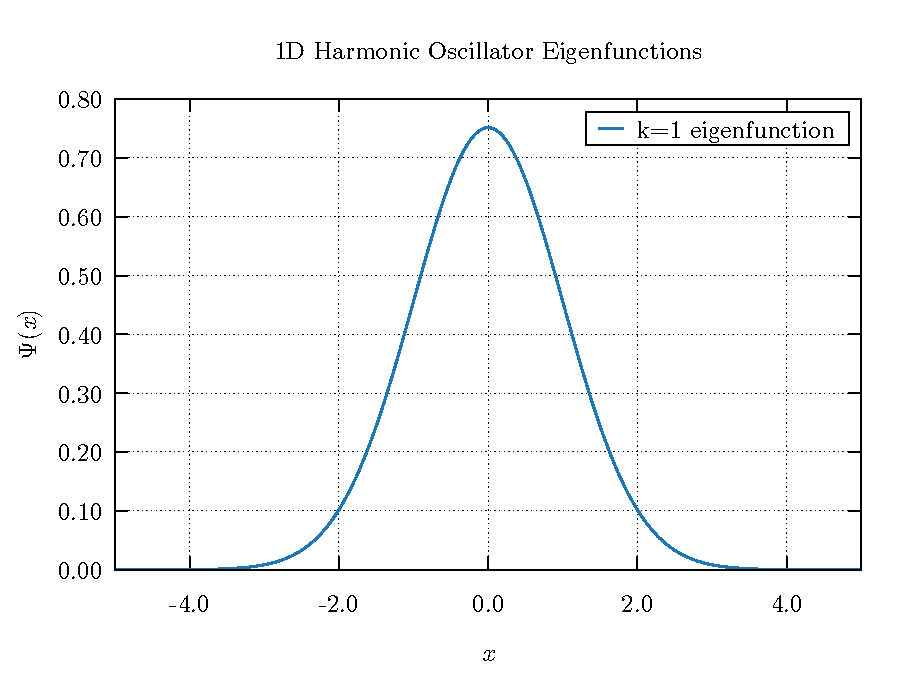
\includegraphics[width=0.48\textwidth]{images/1_eigenfunction.pdf}
        \label{fig:06_R_1}
    }
    \hfill
    \subfloat[][{\small \( k = 2 \)}]{
        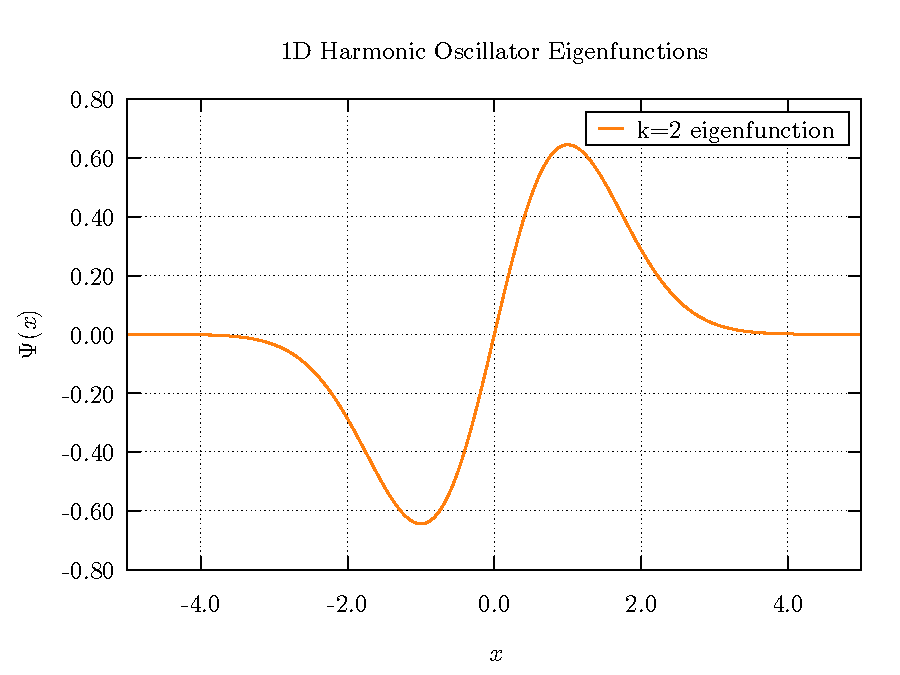
\includegraphics[width=0.48\textwidth]{images/2_eigenfunction.pdf}
        \label{fig:06_R_2}
    }

    \subfloat[][{\small \( k = 3 \)}]{
        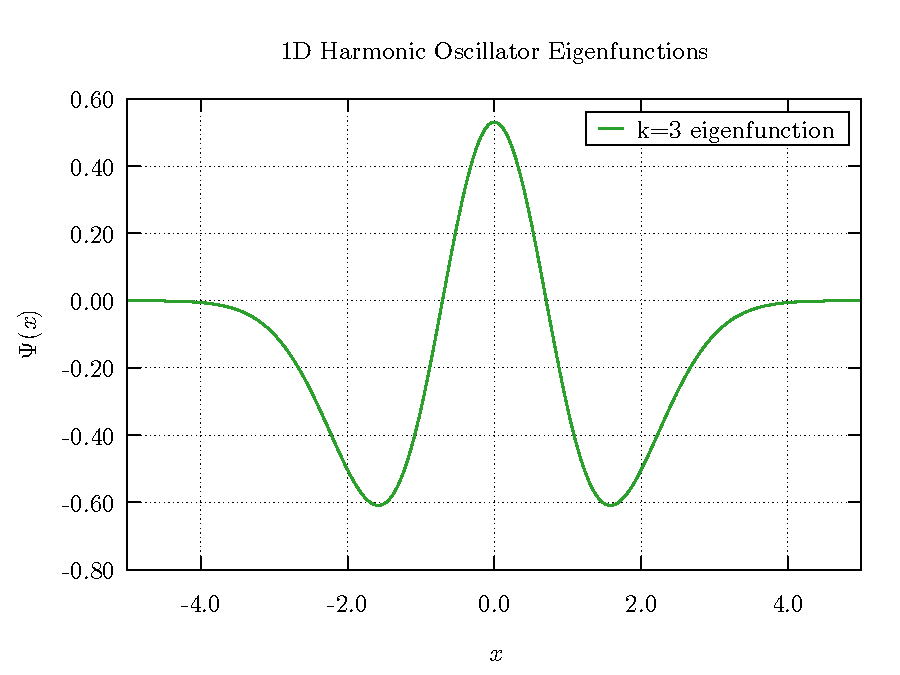
\includegraphics[width=0.48\textwidth]{images/3_eigenfunction.pdf}
        \label{fig:06_R_3}
    }
    \hfill
    \subfloat[][{\small \( k = 4 \)}]{
        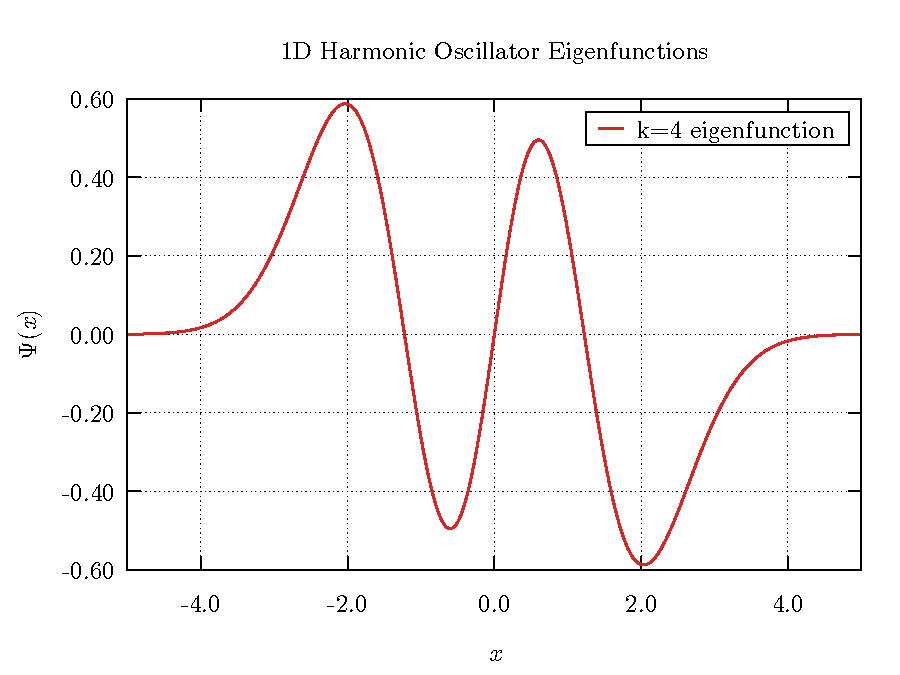
\includegraphics[width=0.48\textwidth]{images/4_eigenfunction.pdf}
        \label{fig:06_R_4}
    }
    \caption{First \( k = 4 \) normalized eigenfunctions obtained from numerical simulation.}
    \label{fig:04_R_1234}
\end{figure*}

The first \( (N+1) \) numerical eigenvalues, with \( N = 2500 \), are computed and compared with the theoretical expectation in Eq. \ref{eq:06_T_2}. The relative error between numerical and theoretical computations is showed in Figure \ref{fig:06_R_5}, where it is plotted for every \( E_{k} \), with \( 0 < k \le 2500 \). We can see how the numerical solution through the finite differences method is approximately correct up to \( k \sim 10 \), then the \( E_{k,\mathrm{num}} \)s start to explode.

\begin{figure}[!h]
    \centering
    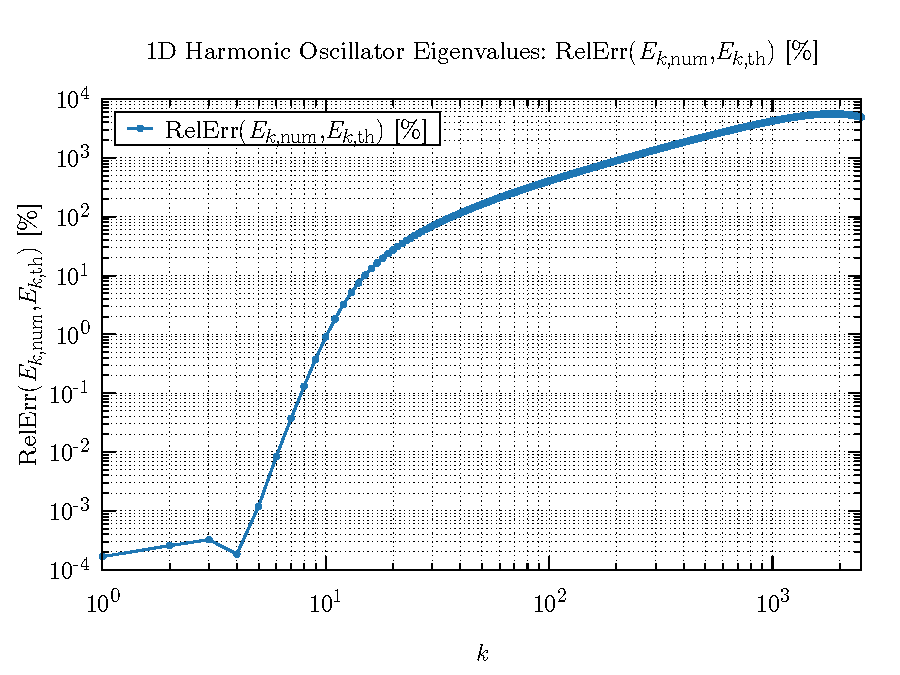
\includegraphics[width=0.5\textwidth]{images/eigenvalues.pdf}
    \caption{\label{fig:06_R_5} Relative error \( \frac{\abs{E_{k,\mathrm{num}} - E_{k,\mathrm{th}}}}{E_{k,\mathrm{th}}} \) for \( 0 < k \le 2500 \).}
\end{figure}


\section{Self-evaluation}
In this work we managed to solve numerically the time independent Schr$\mathrm{\ddot{o}}$dinger equation for a monodimensional harmonic oscillator in a limited space interval. This task is accomplished using a finite differences method and Lapack functions for the code implementation of the diagonalization of a tridiagonal matrix, representing the discretized Hamiltonian.

Concerning the priorities for a good scientific software, the code implemented has the following features:
\begin{itemize}
    \item \textbf{correctness}: the numerical solutions for the first \( k \) eigenvalues and eigenfunctions, with \( k \sim 10 \), is in agreement with theory with good precision;
    \item \textbf{numerical stability}: small variations in the input arguments of the main program do not result in catastrophic variations in the output;
    \item \textbf{accurate discretization}: the step size can be set to a sufficiently small size to capture the physics of the problem, but this is possible only for the first \( k \sim 10 \) eigenvalues, since the method employed has a finite order of precision;
    \item \textbf{flexibility}: the code implementation allows to run the numerical simulation for different values of \( m \), \( \omega \) parameters, to control the discretization and the size of the space interval in which the simulation is run. The next step to further improve this feature is adding an argument parser;
    \item \textbf{efficiency}: state-of-the-art tools like Lapack functions are employed for the most critical steps of the simulation. However, a deeper analysis on the optimal work parameters of the diagonalization functions should be done.
\end{itemize}

\end{document}
